\documentclass[oneside,a4paper,14pt]{extreport}

% Font tiếng Việt
\usepackage[T5]{fontenc}
\usepackage[utf8]{inputenc}
\DeclareTextSymbolDefault{\DH}{T1}

% equation
\usepackage{breqn}
\usepackage{amsfonts}
\usepackage{bm}

% Tài liệu tham khảo
\usepackage[
	sorting=nty,
	backend=bibtex,
	defernumbers=true]{biblatex}
\usepackage[unicode]{hyperref} % Bookmark tiếng Việt
\addbibresource{References/references.bib}

\makeatletter
\def\blx@maxline{77}
\makeatother

% Chèn hình, các hình trong luận văn được để trong thư mục tab_img/
\usepackage{graphicx}
\usepackage{caption}
\usepackage{subcaption}
\graphicspath{ {tab_img/} }

% Chèn và định dạng mã nguồn
\usepackage{listings}
\usepackage{color}
\definecolor{codegreen}{rgb}{0,0.6,0}
\definecolor{codegray}{rgb}{0.5,0.5,0.5}
\definecolor{codepurple}{rgb}{0.58,0,0.82}
\definecolor{backcolour}{rgb}{0.95,0.95,0.92}
\lstdefinestyle{mystyle}{
    backgroundcolor=\color{backcolour},   
    commentstyle=\color{codegreen},
    keywordstyle=\color{magenta},
    numberstyle=\tiny\color{codegray},
    stringstyle=\color{codepurple},
    basicstyle=\footnotesize,
    breakatwhitespace=false,         
    breaklines=true,                 
    captionpos=b,                    
    keepspaces=true,                 
    numbers=left,                    
    numbersep=5pt,                  
    showspaces=false,                
    showstringspaces=false,
    showtabs=false,                  
    tabsize=2
}
\lstset{style=mystyle}

% Chèn và định dạng mã giả
\usepackage{amsmath}
\usepackage{algorithm}
\usepackage[noend]{algpseudocode}
\makeatletter
\def\BState{\State\hskip-\ALG@thistlm}
\makeatother

% chèn inline code
\usepackage{xparse}
\NewDocumentCommand{\codeword}{v}{%
    \texttt{\textcolor{blue}{#1}}%
}

% Bảng biểu
\usepackage{multirow}
\usepackage{rotating}
\usepackage{vcell}
\usepackage{array}
\usepackage{diagbox}
\usepackage{booktabs}
\usepackage{colortbl}
\newcolumntype{L}[1]{>{\raggedright\let\newline\\\arraybackslash\hspace{0pt}}m{#1}}
\newcolumntype{C}[1]{>{\centering\let\newline\\\arraybackslash\hspace{0pt}}m{#1}}
\newcolumntype{R}[1]{>{\raggedleft\let\newline\\\arraybackslash\hspace{0pt}}m{#1}}

% Đổi tên mặc định
\renewcommand{\chaptername}{Chương}
\renewcommand{\figurename}{Hình}
\renewcommand{\tablename}{Bảng}
\renewcommand{\contentsname}{Mục lục}
\renewcommand{\listfigurename}{Danh sách hình}
\renewcommand{\listtablename}{Danh sách bảng}
\renewcommand{\appendixname}{Phụ lục}

% Định dạng chapter
\usepackage{titlesec}
\titleformat{\chapter}
    [display] 
    {\normalfont\bfseries\Large}{\chaptername \ \thechapter}{10pt}{\huge}
\titlespacing*{\chapter}{0pt}{-10pt}{40pt} %khoảng cách giữa chapter và đầu trang

\titleformat{\section}
    {\normalfont\bfseries\large}{\thesection}{1em}{}

\titleformat{\subsection}
    {\normalfont\bfseries\normalsize}{\thesubsection}{1em}{}

% Dãn dòng 1.5
\usepackage{setspace}
\onehalfspacing

% Thụt vào đầu dòng
\usepackage{indentfirst}

% Canh lề
\usepackage[
    top=20mm,
    bottom=10mm,
    left=30mm,
    right=20mm,
    footskip = 15mm,
    includefoot]{geometry}

% Trang bìa
\usepackage{tikz}
\usetikzlibrary{calc}
\newcommand\HRule{\rule{\textwidth}{1pt}}

\begin{document}

\begin{table}[H]
    \centering
    \caption*{Bảng kết quả (\%) của mô hình huấn luyện tập trung và phân tán (FedAvg, dữ liệu IID) trên MNIST và CIFAR-10}
    \resizebox{\linewidth}{!}{%
    \begin{tabular}{c|c|ccccc} 
    \toprule
                                  &          & $acc_{micro}$ & $acc_{macro}$ & $P_{macro}$  & $R_{macro}$  & $F1_{macro}$  \\ 
    \hline
    \multirow{2}{*}{MNIST}  & Centralized    & \textbf{97.07}& -             &\textbf{97.04}&\textbf{97.03}& \textbf{97.04}         \\
                            & FedAvg (IID)   &  90.36         & 90.34±2.24     & 90.37±2.29    & 90.25±2.22    & 90.12±2.29  \\
    \hline
    \multirow{2}{*}{CIFAR-10}     & Centralized    & \textbf{61.91} & -              & \textbf{61.7} & \textbf{62.01}& \textbf{61.72}          \\ 
                                  & FedAvg (IID)   & 53.83          &   53.83±3.14   & 53.46±3.19    & 53.85±3.26    & 53±3.21  \\
    \bottomrule
    \end{tabular}
    }
\end{table}

\begin{table}[H]
    \centering
    \caption*{Bảng kết quả (\%) trên người dùng cục bộ của tập dữ liệu MNIST}
    \resizebox{\linewidth}{!}{%
    \begin{tabular}{l|ccccc} 
    \toprule
    \multicolumn{1}{c|}{}          & $acc_{micro}$     & $acc_{macro}$           & $P_{macro}$             & $R_{macro}$             & $F1_{macro}$             \\ 
    \hline
    FedAvg                         & 85.03           & 82.14±14.76           & 82.03±13.88           & 81.54±14.33           & 79.43±16.83            \\
    FedPer                         & 77.29           & 75.48±14.84           & 76.07±14.99           & 74.01±15.13           & 72.32±15.99            \\
    FedAvgMeta                     & 84.84           & 81.56±16.68           & 80.71±17.02           & 81.18±16.16           & 78.31±19.8             \\
    FedPerMeta                     & 75.91           & 74.11±16.2            & 75.68±15.94           & 72.93±15.58           & 71.22±16.77            \\
    FedMeta(MAML)                  & 92.99           & 91.14±5.99           & 90.56±6.24           & 90.98±5.9            & 90.16±6.28            \\
    FedMeta(Meta-SGD)              & 98.02           & 96.35±4.62           & 96.49±4.1            & 95.64±5.94           & 95.80±5.51            \\
    \textbf{FedMeta-Per(MAML)}     & \textbf{99.37 } & \textbf{99.12±1.29 } & \textbf{99.11±1.3  } & \textbf{98.82±1.99 } & \textbf{98.94±1.6}  \\
    \textbf{FedMeta-Per(Meta-SGD)} & 98.92           & 98.15±3.32           & 98.42±1.95           & 98.42±1.96           & 98.20±2.94            \\
    \bottomrule
    \end{tabular}
    }
\end{table}

\begin{table}[H]
    \centering
    \caption*{Bảng kết quả (\%) trên người dùng mới của tập dữ liệu MNIST}
    \resizebox{\linewidth}{!}{%
    \begin{tabular}{l|ccccc} 
    \toprule
    \multicolumn{1}{c|}{} & $acc_{micro}$  & $acc_{macro}$         & $P_{macro}$           & $R_{macro}$           & $F1_{macro}$           \\ 
    \hline
    FedAvg                & 83.92          & 81.69±19.71          & 79.57±20.18          & 80.46±17.84          & 77.66±22.54           \\
    FedPer                & 78.3           & 76.19±18.79          & 75.91±17.52          & 74.73±17.32          & 72.72±19.3            \\
    FedAvgMeta            & 84.34          & 82.37±17.42          & 81.38±16.25          & 80.91±15.62          & 78.78±19.31           \\
    FedPerMeta            & 77.47          & 75.56±20.33          & 75.09±19.52          & 74.92±18.85          & 72.60±21.37           \\
    FedMeta(MAML)         & 92.96          & 91.88±5.88          & 90.14±7.97          & 90.74±5.95          & 90.02±7.34           \\
    FedMeta(Meta-SGD)     & 96.39          & 93.53±8.39          & 93.73±10.26          & 88.65±14.06          & 89.31±14.56           \\
    \textbf{FedMeta-Per(MAML)}     & 93.6           & 93.57±5.58          & 93.64±5.56          & 90.98±6.98          & 91.83±6.43           \\
    \textbf{FedMeta-Per(Meta-SGD)} & \textbf{96.62} & \textbf{95.88±3.58} & \textbf{95.73±4.11} & \textbf{94.34±5.05} & \textbf{94.85±4.61}  \\
    \bottomrule
    \end{tabular}
    }
\end{table}

\clearpage

\begin{table}[H]
    \centering
    \caption*{Bảng kết quả (\%) trên người dùng cục bộ của tập dữ liệu CIFAR-10}
    \resizebox{\linewidth}{!}{%
    \begin{tabular}{l|ccccc} 
    \toprule
    \multicolumn{1}{c|}{}          & $acc_{micro}$  & $acc_{macro}$          & $P_{macro}$            & $R_{macro}$            & $F1_{macro}$       \\ 
    \hline
    FedAvg                         & 19.02         & 19.29±25.11          & 15.57±23.7           & 20.65±25.55          & 16.85±23.92           \\
    FedPer                         & 13.22         & 12.99±19.39          & 18.34±28.59          & 14.14±20.83          & 10.52±14.91           \\
    FedAvgMeta                     & 40.3          & 38.47±31.52          & 32.84±32.06          & 39.33±30.35          & 33.81±30.61           \\
    FedPerMeta                     & 18.57         & 17.48±22.55          & 20.02±27.4           & 18.43±23.47          & 14.54±18.67           \\
    FedMeta(MAML)                  & 69.02         & 68.76±14.86          & 67.42±21.16          & 66.56±13.48          & 61.14±20           \\
    FedMeta(Meta-SGD)              & 78.63         & 78.73±11.59          & 74.65±21.12          & 75.25±14.09          & 72.87±18.31           \\
    \textbf{FedMeta-Per(MAML)}     & \textbf{86.6} & \textbf{86.52±6.31} & \textbf{86.43±5.88} & \textbf{85.47±6.87} & \textbf{85.33±6.77}  \\
    \textbf{FedMeta-Per(Meta-SGD)} & 85.61         & 85.68±7.22          & 86.26±6.35          & 85.36±6.83          & 85.08±7.32           \\
    \bottomrule
    \end{tabular}
    }
\end{table}

\begin{table}[H]
    \centering
    \caption*{Bảng kết quả (\%) trên người dùng mới của tập dữ liệu CIFAR-10}
    \resizebox{\linewidth}{!}{%
    \begin{tabular}{l|ccccc} 
    \toprule
    \multicolumn{1}{c|}{}          & $acc_{micro}$   & $acc_{macro}$          & $P_{macro}$            & $R_{macro}$            & $F1_{macro}$            \\ 
    \hline
    FedAvg                         & 24.63          & 24.83±22.57          & 18.36±20.15            & 24.44±21.95          & 20.52±20.45           \\
    FedPer                         & 14.4           & 14.52±20.15          & 12.59±20.65            & 14.23±19.58          & 10.66±13.79           \\
    FedAvgMeta                     & 43.39          & 43.54±18             & 33.45±21.44            & 42.87±16.98          & 35.14±17.22           \\
    FedPerMeta                     & 13.33          & 13.57±19.62          & 11.99±19.52            & 13.53±19.08          & 10.05±13.17           \\
    FedMeta(MAML)                  & 61.69          & 61.64±12.49          & 52.66±26.06            & 59.94±12.35          & 50.76±19.2            \\
    FedMeta(Meta-SGD)              & 68.36          & 67.89±15.11          & \textbf{70.3±22.37} & 66.86±15.02          & 60.24±21.52           \\
    \textbf{FedMeta-Per(MAML)}     & 64.22          & 63.70±12.29          & 57.06±24.99            & 61.63±12.66          & 53.68±19.06           \\
    \textbf{FedMeta-Per(Meta-SGD)} & \textbf{69.97} & \textbf{69.13±14.63} & 66.53±24.91          & \textbf{67.82±15.34} & \textbf{62.42±20.94}  \\
    \bottomrule
    \end{tabular}
    }
\end{table}

\clearpage

\begin{sidewaysfigure}
    \centering
    \begin{subfigure}{\textwidth}
        \centering
        \begin{subfigure}{.5\textwidth}
            \centering
            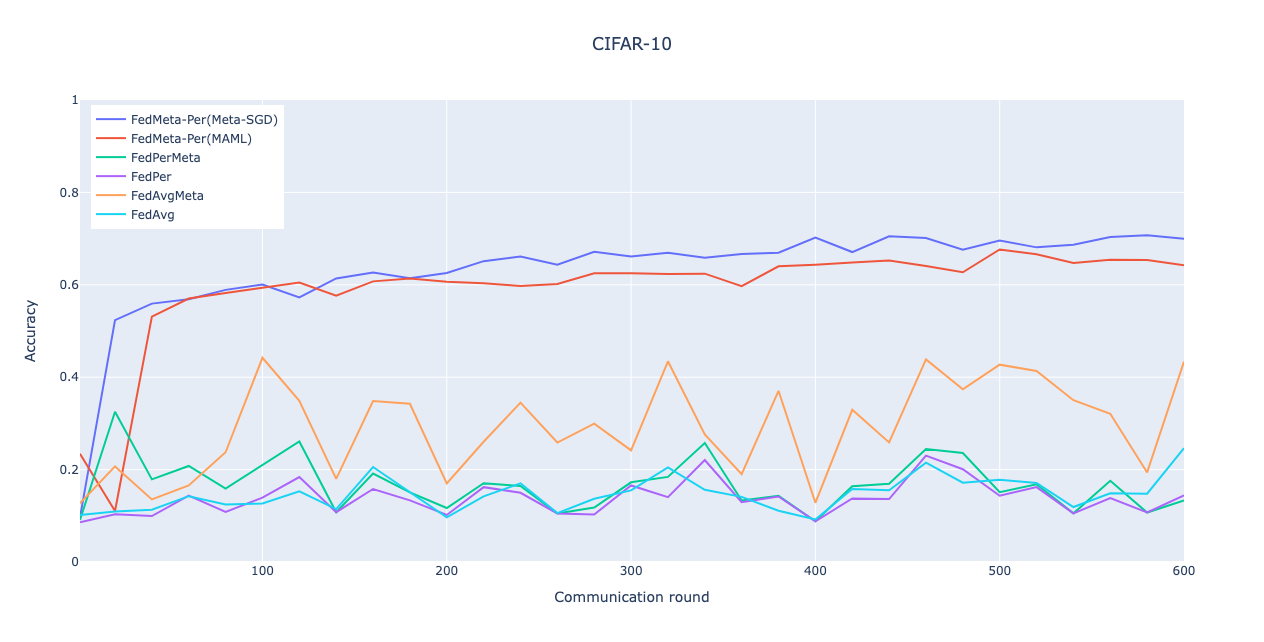
\includegraphics[width=\linewidth]{./tab_img/cifar_per_new.png}
            \caption{CIFAR-10, new clients}
            \label{fig:cifar_per_new}
        \end{subfigure}%
        \begin{subfigure}{.5\textwidth}
            \centering
            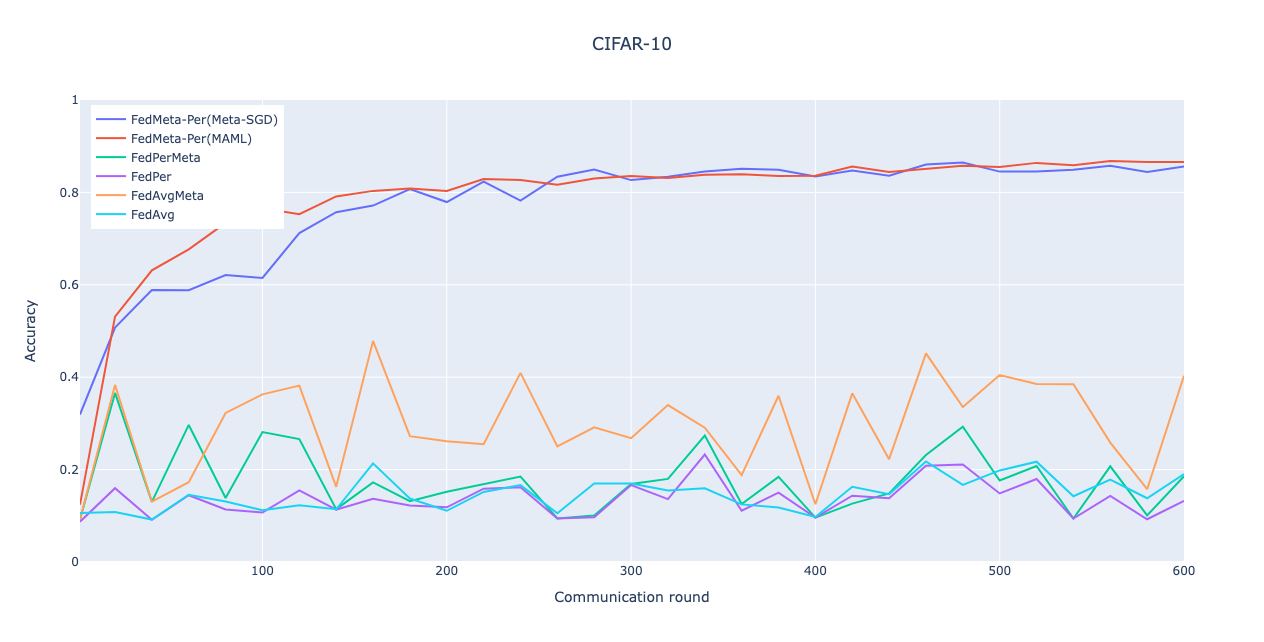
\includegraphics[width=\linewidth]{./tab_img/cifar_per_old.png}
            \caption{CIFAR-10, local clients}
            \label{fig:cifar_per_old}
        \end{subfigure}
        % \caption{A figure with two subfigures}
        % \label{fig:test}
    \end{subfigure}

    \begin{subfigure}{\textwidth}
        \centering
        \begin{subfigure}{.5\textwidth}
            \centering
            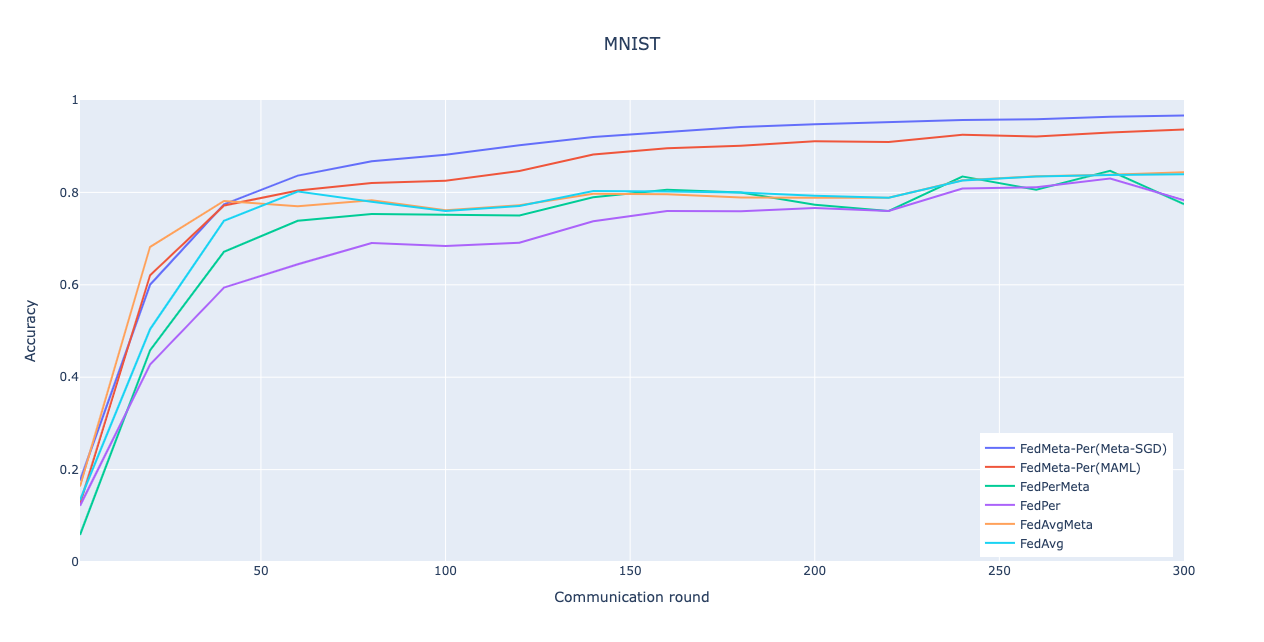
\includegraphics[width=\linewidth]{./tab_img/mnist_per_new.png}
            \caption{MNIST, new clients}
            \label{fig:mnist_per_new}
        \end{subfigure}%
        \begin{subfigure}{.5\textwidth}
            \centering
            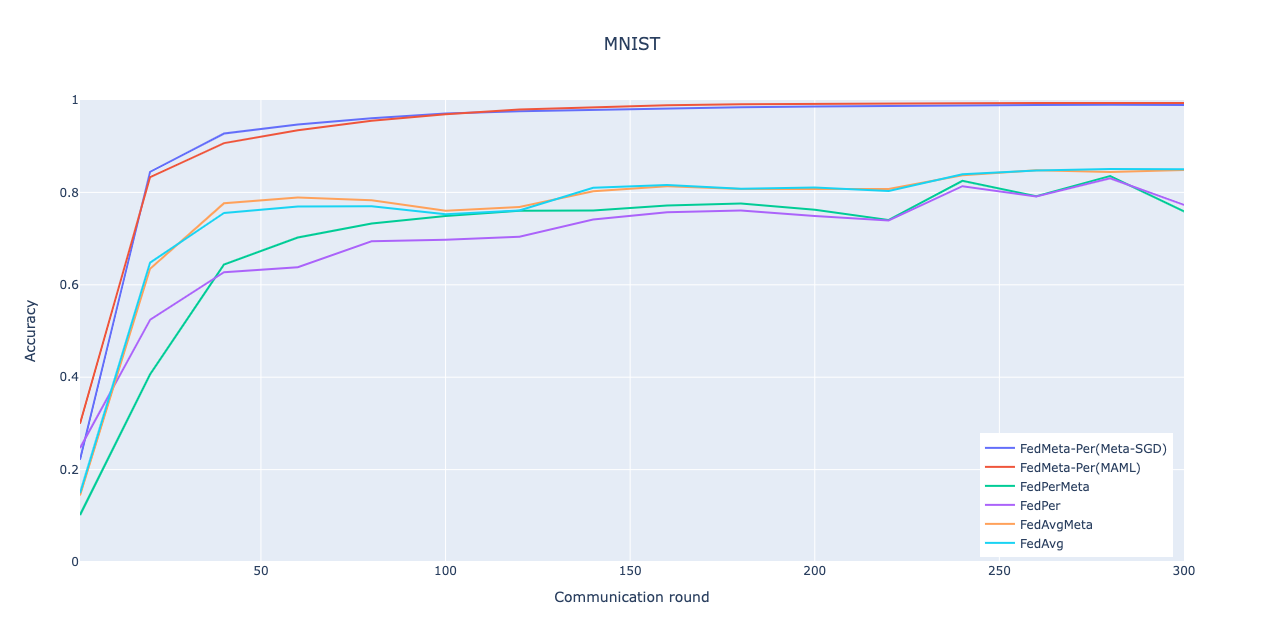
\includegraphics[width=\linewidth]{./tab_img/mnist_per_old.png}
            \caption{MNIST, local clients}
            \label{fig:mnist_per_old}
        \end{subfigure}
        % \caption{A figure with two subfigures}
        % \label{fig:test}
    \end{subfigure}
    \caption*{FedMeta-Per vs. (FedAvg, FedAvgMeta, FedPer, FedPerMeta)}
    \label{fig:fedper_acc}
\end{sidewaysfigure}

\begin{sidewaysfigure}
    \centering
    \begin{subfigure}{\textwidth}
        \centering
        \begin{subfigure}{.5\textwidth}
            \centering
            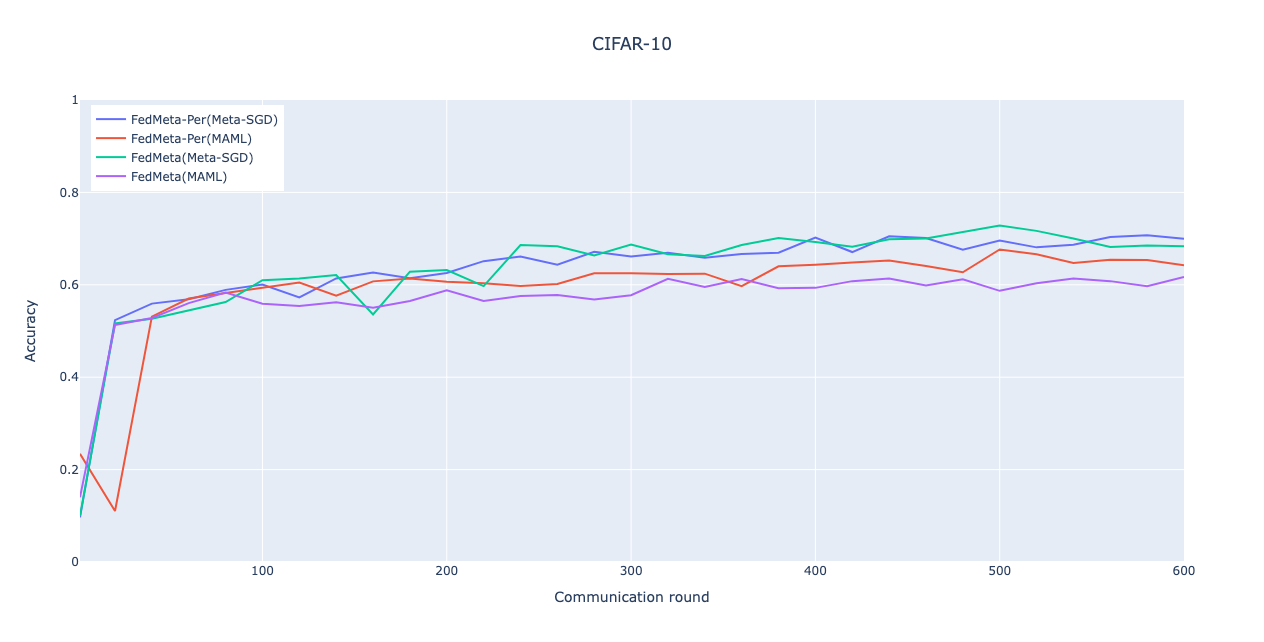
\includegraphics[width=\linewidth]{./tab_img/cifar_meta_new.png}
            \caption{CIFAR-10, new clients}
            \label{fig:cifar_meta_new}
        \end{subfigure}%
        \begin{subfigure}{.5\textwidth}
            \centering
            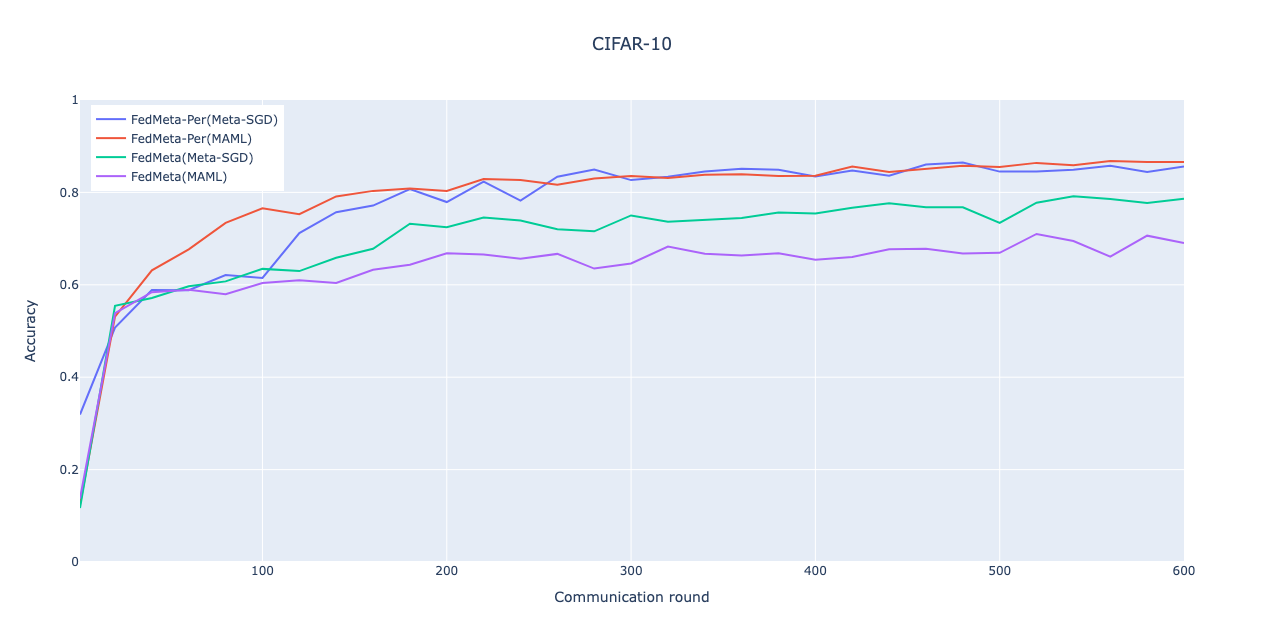
\includegraphics[width=\linewidth]{./tab_img/cifar_meta_old.png}
            \caption{CIFAR-10, local clients}
            \label{fig:cifar_meta_old}
        \end{subfigure}
        % \caption{A figure with two subfigures}
        % \label{fig:test}
    \end{subfigure}

    \begin{subfigure}{\textwidth}
        \centering
        \begin{subfigure}{.5\textwidth}
            \centering
            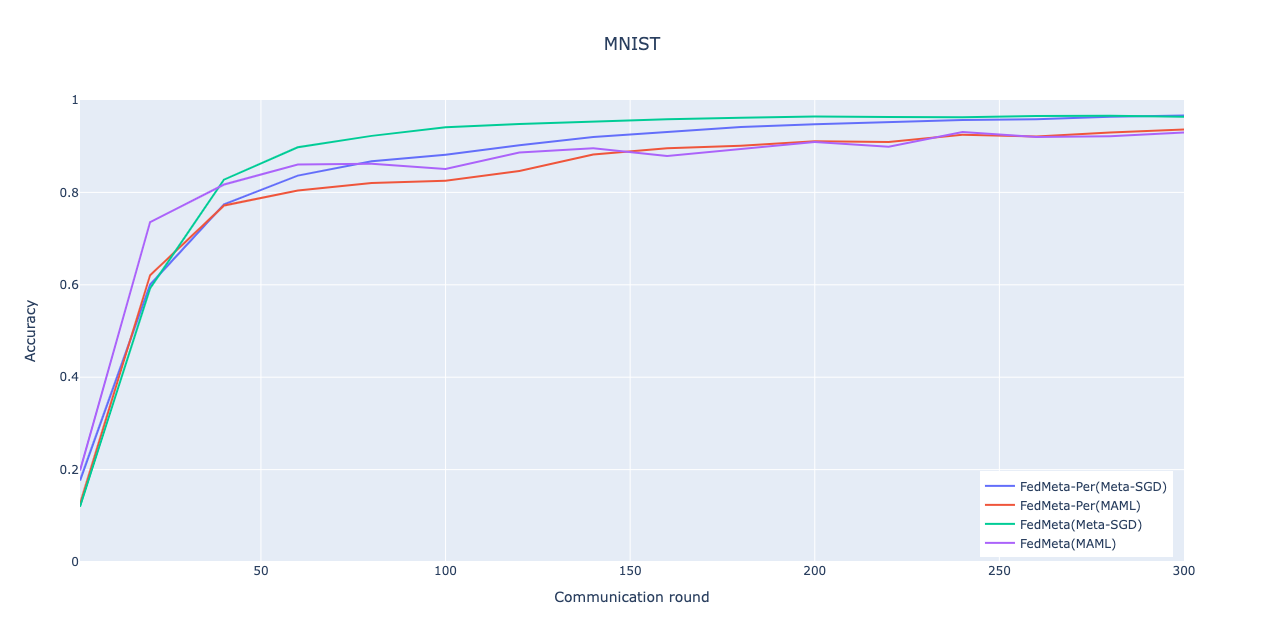
\includegraphics[width=\linewidth]{./tab_img/mnist_meta_new.png}
            \caption{MNIST, new clients}
            \label{fig:mnist_meta_new}
        \end{subfigure}%
        \begin{subfigure}{.5\textwidth}
            \centering
            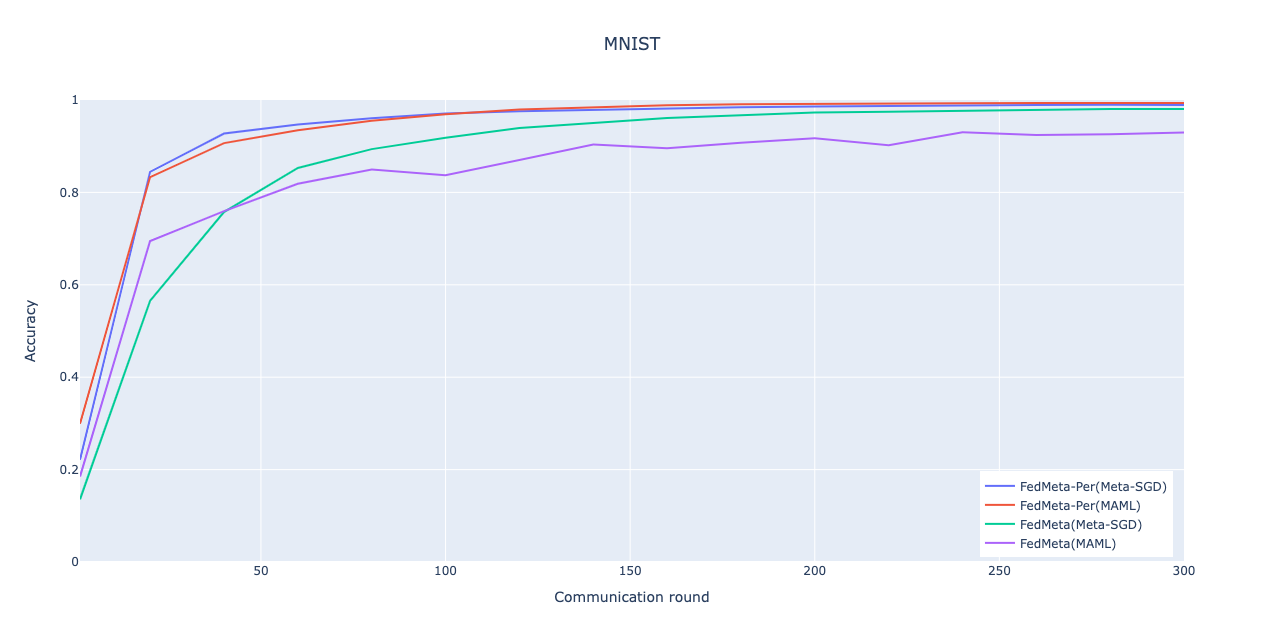
\includegraphics[width=\linewidth]{./tab_img/mnist_meta_old.png}
            \caption{MNIST, local clients}
            \label{fig:mnist_meta_old}
        \end{subfigure}
        % \caption{A figure with two subfigures}
        % \label{fig:test}
    \end{subfigure}
    \caption*{FedMeta-Per vs. FedMeta}
    \label{fig:fedmeta_acc}
\end{sidewaysfigure}

\begin{table}[H]
    \centering
    \caption{Bảng kết quả (\%) trên tập dữ liệu CIFAR-10}
    \label{tab:cifar}
    \resizebox{\linewidth}{!}{%
    \begin{tabular}{c|l|ccccc} 
    \toprule
    \multicolumn{1}{l}{}                             & \multicolumn{1}{c|}{}                   & $acc_{micro}$   & $acc_{macro}$        & $P_{macro}$         & $R_{macro}$          & $F1_{macro}$         \\ 
    \hline
    \multirow{8}{*}{local client}                    & FedAvg                                  & 19.02         & 19.29±25.11          & 15.57±23.7           & 20.65±25.55          & 16.85±23.92           \\
                                                     & FedPer                                  & 13.22         & 12.99±19.39          & 18.34±28.59          & 14.14±20.83          & 10.52±14.91           \\
                                                     & FedAvgMeta                              & 40.3          & 38.47±31.52          & 32.84±32.06          & 39.33±30.35          & 33.81±30.61           \\
                                                     & FedPerMeta                              & 18.57         & 17.48±22.55          & 20.02±27.4           & 18.43±23.47          & 14.54±18.67           \\
                                                     & FedMeta(MAML)                           & 69.02         & 68.76±14.86          & 67.42±21.16          & 66.56±13.48          & 61.14±20              \\
                                                     & FedMeta(Meta-SGD)                       & 78.63         & 78.73±11.59          & 74.65±21.12          & 75.25±14.09          & 72.87±18.31           \\
                                                     & \textbf{FedMeta-Per(MAML)}              & \textbf{86.6} & \textbf{86.52±6.31}  & \textbf{86.43±5.88}  & \textbf{85.47±6.87}  & \textbf{85.33±6.77}   \\
                                                     & \textbf{FedMeta-Per(Meta-SGD)}          & 85.61         & 85.68±7.22           & 86.26±6.35           & 85.36±6.83           & 85.08±7.32            \\
    \hline
    \multicolumn{1}{l|}{\multirow{8}{*}{new client}} & FedAvg                                  & 24.63          & 24.83±22.57          & 18.36±20.15            & 24.44±21.95          & 20.52±20.45           \\
    \multicolumn{1}{l|}{}                            & FedPer                                  & 14.4           & 14.52±20.15          & 12.59±20.65            & 14.23±19.58          & 10.66±13.79           \\
    \multicolumn{1}{l|}{}                            & FedAvgMeta                              & 43.39          & 43.54±18             & 33.45±21.44            & 42.87±16.98          & 35.14±17.22           \\
    \multicolumn{1}{l|}{}                            & FedPerMeta                              & 13.33          & 13.57±19.62          & 11.99±19.52            & 13.53±19.08          & 10.05±13.17           \\
    \multicolumn{1}{l|}{}                            & FedMeta(MAML)                           & 61.69          & 61.64±12.49          & 52.66±26.06            & 59.94±12.35          & 50.76±19.2            \\
    \multicolumn{1}{l|}{}                            & FedMeta(Meta-SGD)                       & 68.36          & 67.89±15.11          & \textbf{70.3±22.37}    & 66.86±15.02          & 60.24±21.52           \\
    \multicolumn{1}{l|}{}                            & \textbf{\textbf{FedMeta-Per(MAML)}}     & 64.22          & 63.70±12.29          & 57.06±24.99            & 61.63±12.66          & 53.68±19.06           \\
    \multicolumn{1}{l|}{}                            & \textbf{\textbf{FedMeta-Per(Meta-SGD)}} & \textbf{69.97} & \textbf{69.13±14.63} & 66.53±24.91            & \textbf{67.82±15.34} & \textbf{62.42±20.94}  \\
    \bottomrule
    \end{tabular}
    }
\end{table}

\begin{table}[H]
    \centering
    \caption{Bảng kết quả (\%) trên tập dữ liệu MNIST}
    \label{tab:mnist}
    \resizebox{\linewidth}{!}{%
    \begin{tabular}{c|l|ccccc} 
    \toprule
    \multicolumn{1}{l}{}                             & \multicolumn{1}{c|}{}                   & $acc_{micro}$   & $acc_{macro}$        & $P_{macro}$         & $R_{macro}$          & $F1_{macro}$         \\ 
    \hline
    \multirow{8}{*}{local client}                    & FedAvg                                  & 85.03           & 82.14±14.76          & 82.03±13.88         & 81.54±14.33          & 79.43±16.83          \\
                                                     & FedPer                                  & 77.29           & 75.48±14.84          & 76.07±14.99         & 74.01±15.13          & 72.32±15.99          \\
                                                     & FedAvgMeta                              & 84.84           & 81.56±16.68          & 80.71±17.02         & 81.18±16.16          & 78.31±19.8           \\
                                                     & FedPerMeta                              & 75.91           & 74.11±16.2           & 75.68±15.94         & 72.93±15.58          & 71.22±16.77          \\
                                                     & FedMeta(MAML)                           & 92.99           & 91.14±5.99           & 90.56±6.24          & 90.98±5.9            & 90.16±6.28           \\
                                                     & FedMeta(Meta-SGD)                       & 98.02           & 96.35±4.62           & 96.49±4.1           & 95.64±5.94           & 95.80±5.51           \\
                                                     & \textbf{FedMeta-Per(MAML)}              & \textbf{99.37 } & \textbf{99.12±1.29 } & \textbf{99.11±1.3 } & \textbf{98.82±1.99 } & \textbf{98.94±1.6}   \\
                                                     & \textbf{FedMeta-Per(Meta-SGD)}          & 98.92           & 98.15±3.32           & 98.42±1.95          & 98.42±1.96           & 98.20±2.94           \\ 
    \hline
    \multicolumn{1}{l|}{\multirow{8}{*}{new client}} & FedAvg                                  & 83.92           & 81.69±19.71          & 79.57±20.18         & 80.46±17.84          & 77.66±22.54          \\
    \multicolumn{1}{l|}{}                            & FedPer                                  & 78.3            & 76.19±18.79          & 75.91±17.52         & 74.73±17.32          & 72.72±19.3           \\
    \multicolumn{1}{l|}{}                            & FedAvgMeta                              & 84.34           & 82.37±17.42          & 81.38±16.25         & 80.91±15.62          & 78.78±19.31          \\
    \multicolumn{1}{l|}{}                            & FedPerMeta                              & 77.47           & 75.56±20.33          & 75.09±19.52         & 74.92±18.85          & 72.60±21.37          \\
    \multicolumn{1}{l|}{}                            & FedMeta(MAML)                           & 92.96           & 91.88±5.88           & 90.14±7.97          & 90.74±5.95           & 90.02±7.34           \\
    \multicolumn{1}{l|}{}                            & FedMeta(Meta-SGD)                       & 96.39           & 93.53±8.39           & 93.73±10.26         & 88.65±14.06          & 89.31±14.56          \\
    \multicolumn{1}{l|}{}                            & \textbf{\textbf{FedMeta-Per(MAML)}}     & 93.6            & 93.57±5.58           & 93.64±5.56          & 90.98±6.98           & 91.83±6.43           \\
    \multicolumn{1}{l|}{}                            & \textbf{\textbf{FedMeta-Per(Meta-SGD)}} & \textbf{96.62}  & \textbf{95.88±3.58}  & \textbf{95.73±4.11} & \textbf{94.34±5.05}  & \textbf{94.85±4.61}  \\
    \bottomrule
    \end{tabular}
    }
\end{table}

\begin{figure}
    \centering
    \begin{subfigure}{1.\textwidth}
        \centering
        \begin{subfigure}{.25\textwidth}
            \centering
            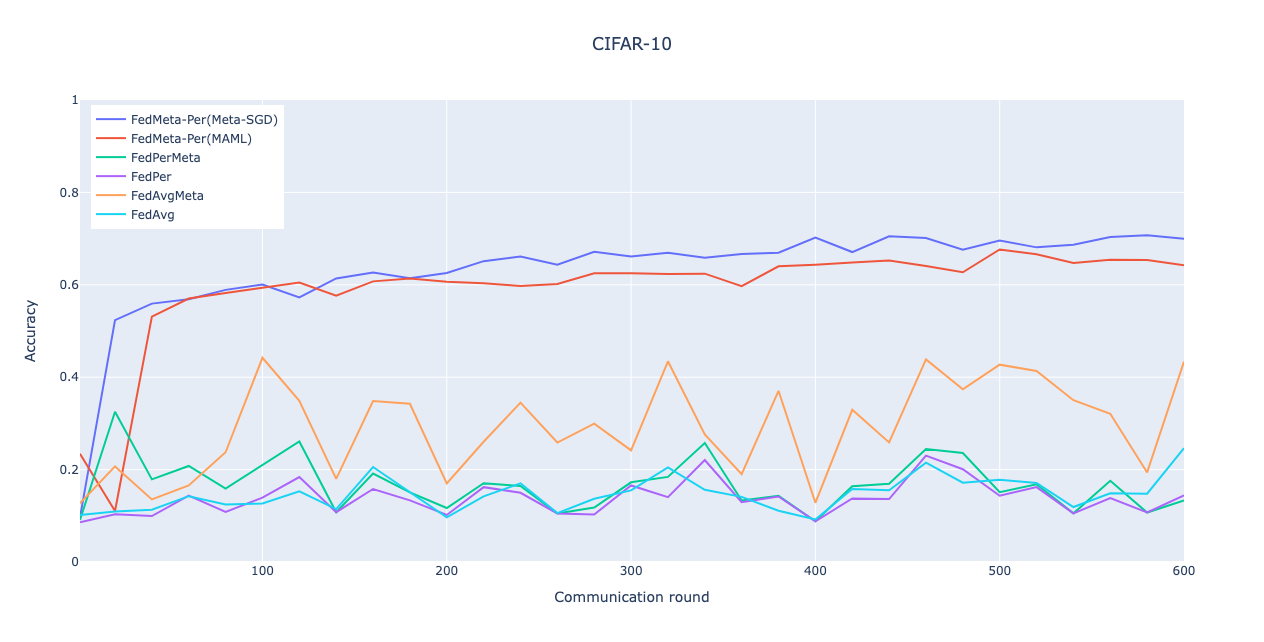
\includegraphics[width=\linewidth]{./tab_img/cifar_per_new.png}
            \caption{CIFAR-10, new clients}
            \label{fig:cifar_per_new}
        \end{subfigure}%
        \begin{subfigure}{.25\textwidth}
            \centering
            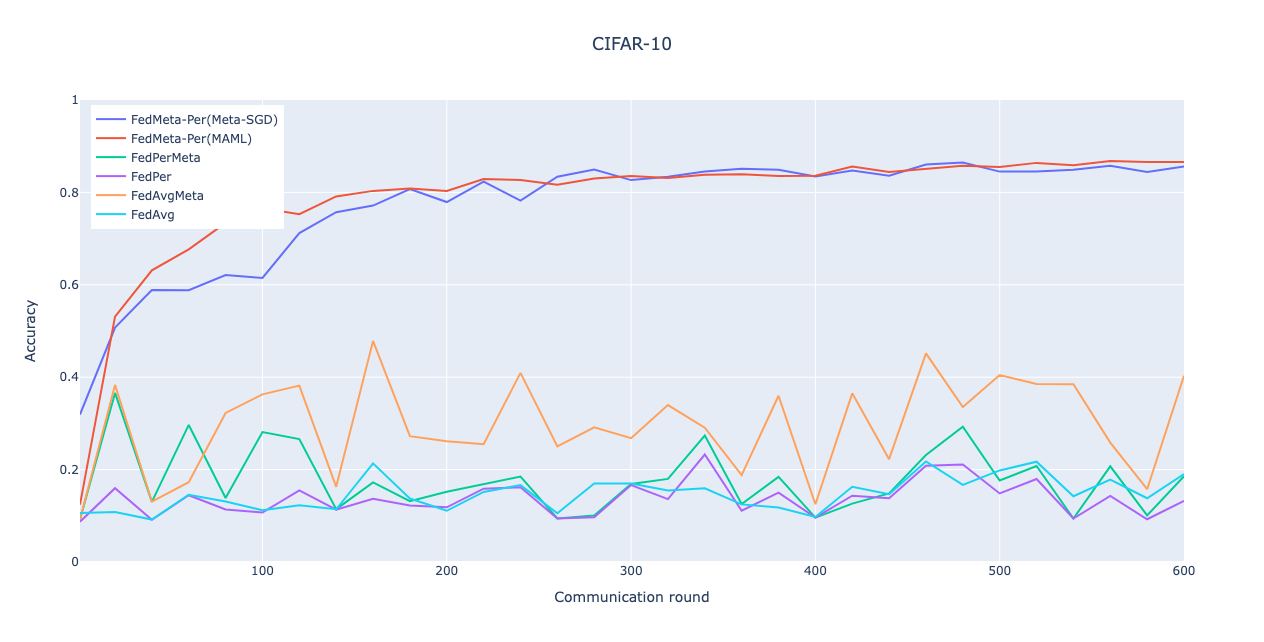
\includegraphics[width=\linewidth]{./tab_img/cifar_per_old.png}
            \caption{CIFAR-10, local clients}
            \label{fig:cifar_per_old}
        \end{subfigure}
        \begin{subfigure}{.25\textwidth}
            \centering
            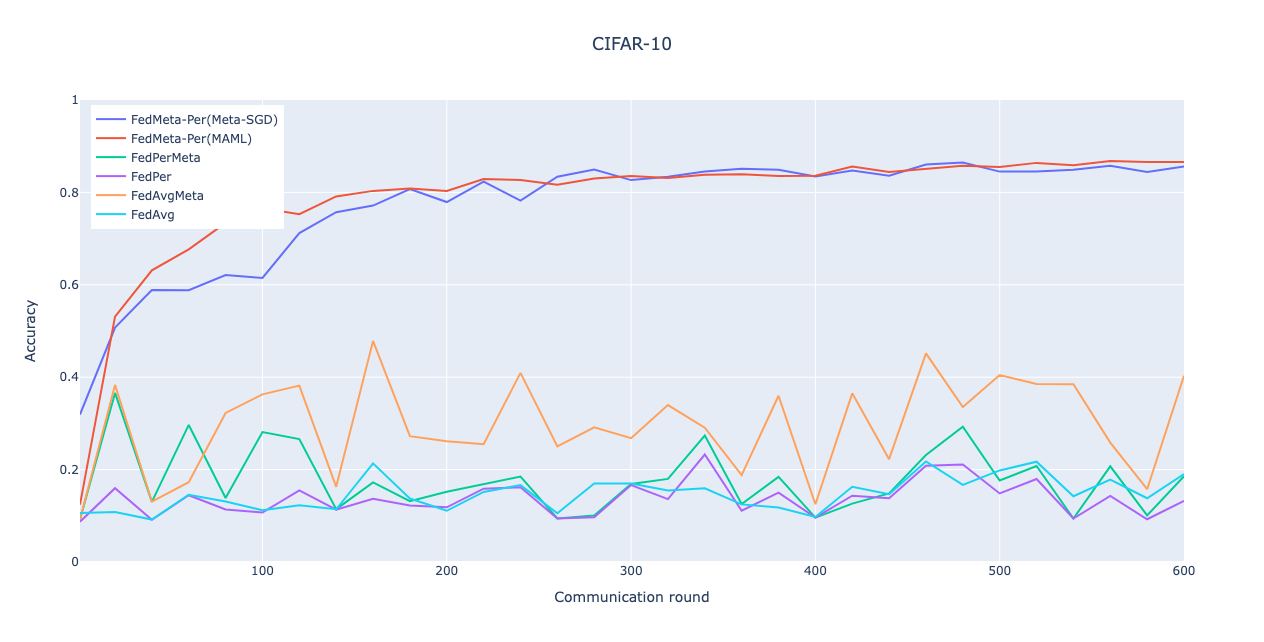
\includegraphics[width=\linewidth]{./tab_img/cifar_per_old.png}
            \caption{CIFAR-10, local clients}
            \label{fig:cifar_per_old}
        \end{subfigure}
        \begin{subfigure}{.25\textwidth}
            \centering
            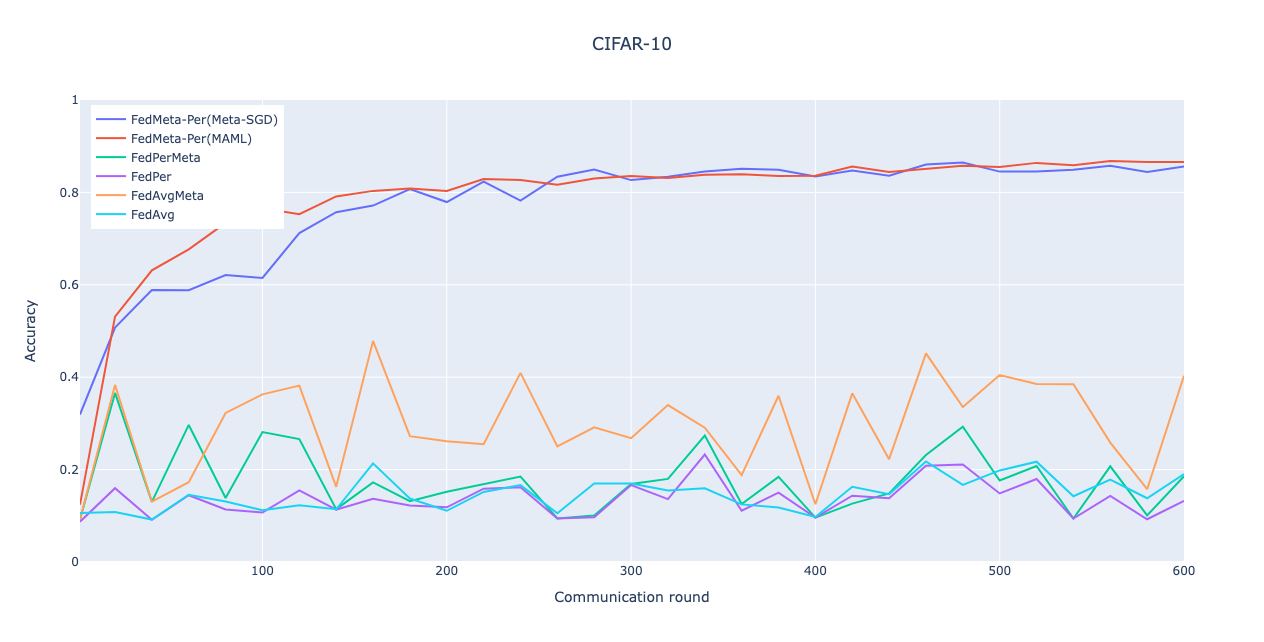
\includegraphics[width=\linewidth]{./tab_img/cifar_per_old.png}
            \caption{CIFAR-10, local clients}
            \label{fig:cifar_per_old}
        \end{subfigure}
        % \caption{A figure with two subfigures}
        % \label{fig:test}
    \end{subfigure}
\end{figure}

\end{document}